\section{Discussion}
\label{sec:slam-discussion}


\subsection{Baseline GLIM Performance Analysis}

The evaluation of the baseline GLIM algorithm revealed two critical failure modes that fundamentally compromised the reliability of its localisation: systematic vertical drift and a catastrophic ``point of no return'' in planar estimation. \cref{tab:baseline_performance} reports the quantitative performance across all datasets.

\subsubsection{Vertical Drift}
The baseline algorithm exhibited systematic drift in the positive altitude ($z$-axis) direction. This drift is illustrated in Dataset 4 (\cref{fig:ds4_z_baseline}), where the vehicle drives a linear trajectory down a vineyard row. Although the actual environment features an elevation gain of approximately 5~m, the baseline GLIM algorithm accumulated nearly 30~m of vertical drift by the end of the row.

This drift demonstrated a self-correcting phenomenon during the return traversal. As the vehicle returned in the opposite direction, the vertical error decreased at a rate symmetrical to its initial accumulation, eventually converging back to the ground truth trajectory at the start of the row. This behaviour suggests that the initial drift was effectively encoded into the generated LiDAR map. During the return pass, the scan-matching process was constrained by this previously mapped geometry. Consequently, the odometry ``undid'' the accumulated drift by aligning the current scans with the erroneous elevation of the existing map. 

This vertical distortion of the map did not appear to hinder subsequent scan matching or loop closure. The algorithm remained capable of registering scans against a map with smooth but substantial Z-axis distortion. This resilience may be a byproduct of the specific environment, characterised by repetitive A-B linear paths with minimal lateral movement—which allows the scan matcher to maintain strong geometric overlap in the X-Y plane despite vertical inconsistencies.

\subsubsection{Planar Drift}
In contrast to the recoverable nature of vertical drift, errors in the X-Y plane frequently led to catastrophic, irrecoverable failure. This ``point of no return'' is most evident in \cref{fig:ds0_xy_baseline}, where the baseline algorithm maintains high accuracy for the first half of the traversal before experiencing a sudden, exponential increase in error. 

At this threshold, the accumulated planar drift distorts the LiDAR map to such an extent that subsequent scan matching becomes unreliable. After this occurs, the trajectory becomes increasingly jagged and stochastic, likely caused by false-positive scan matches that introduce large, discontinuous jumps in the pose estimation and map structure. 

This failure mode is particularly prevalent in the structured and repetitive environments of vineyard rows. Small angular or lateral drifts cause parallel rows in the LiDAR map to diverge or overlap incorrectly. Once this map distortion exceeds the scan matcher's convergence radius, the algorithm may incorrectly register the vehicle's current scan against an adjacent row. This ``row-skipping'' effect creates a feedback loop of map corruption, where each incorrect match further distorts the global map, making recovery unlikely for the remainder of the trajectory, as illustrated in \cref{fig:row-skip-baseline}.

\begin{figure}[htbp]
    \centering
    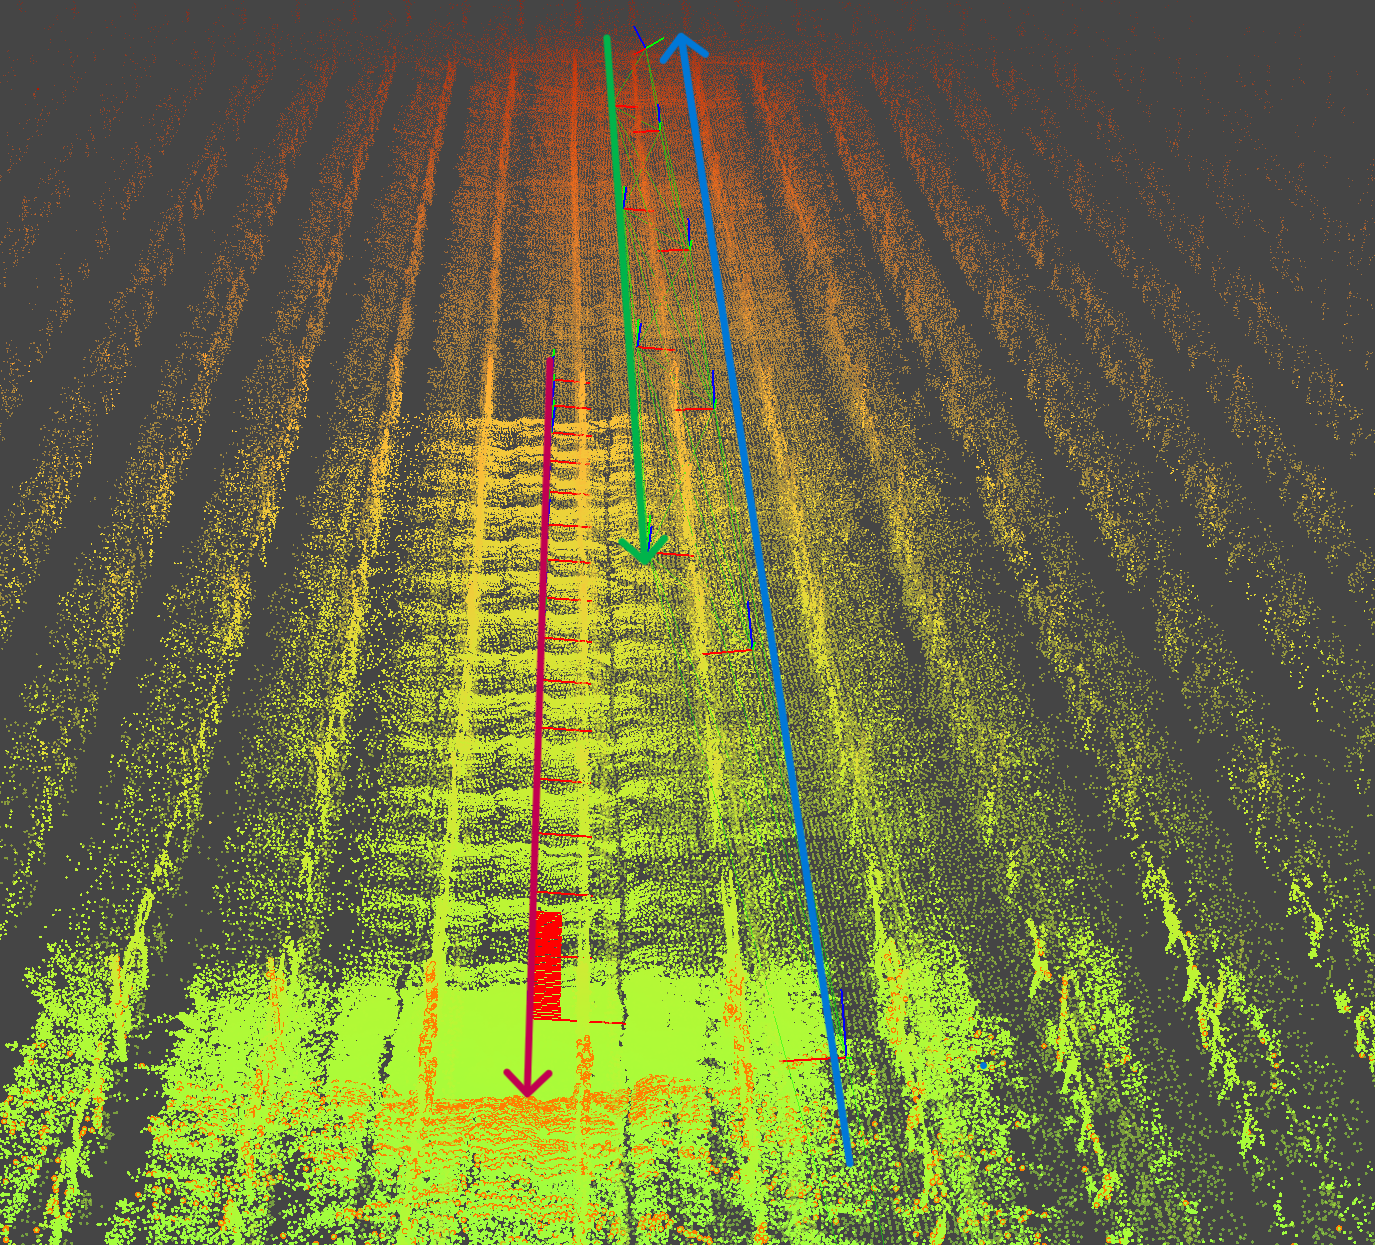
\includegraphics[width=0.85\linewidth]{3-SLAM/3-discussion/figures/row_jump.png}
    \caption{Row-skipping failure exhibited by the baseline GLIM SLAM. The blue arrow (right) shows the robot trajectory up the row. The green arrow (centre) shows the correct return traversal down the adjacent row. Approximately mid-row, the estimated trajectory abruptly shifts one lane to the left (red arrow), where scan matching has falsely converged against the geometry of the neighbouring row.}
    \label{fig:row-skip-baseline}
\end{figure}

The inherent self-similarity driving this failure is visible in the raw LiDAR map: as shown in \cref{fig:zoomedRowsSLAMMap}, the vineyard rows are geometrically indistinguishable from one another, confirming that the corridor-like structure provides no longitudinal discriminability for the scan matcher.

\begin{figure}[htbp]
    \centering
    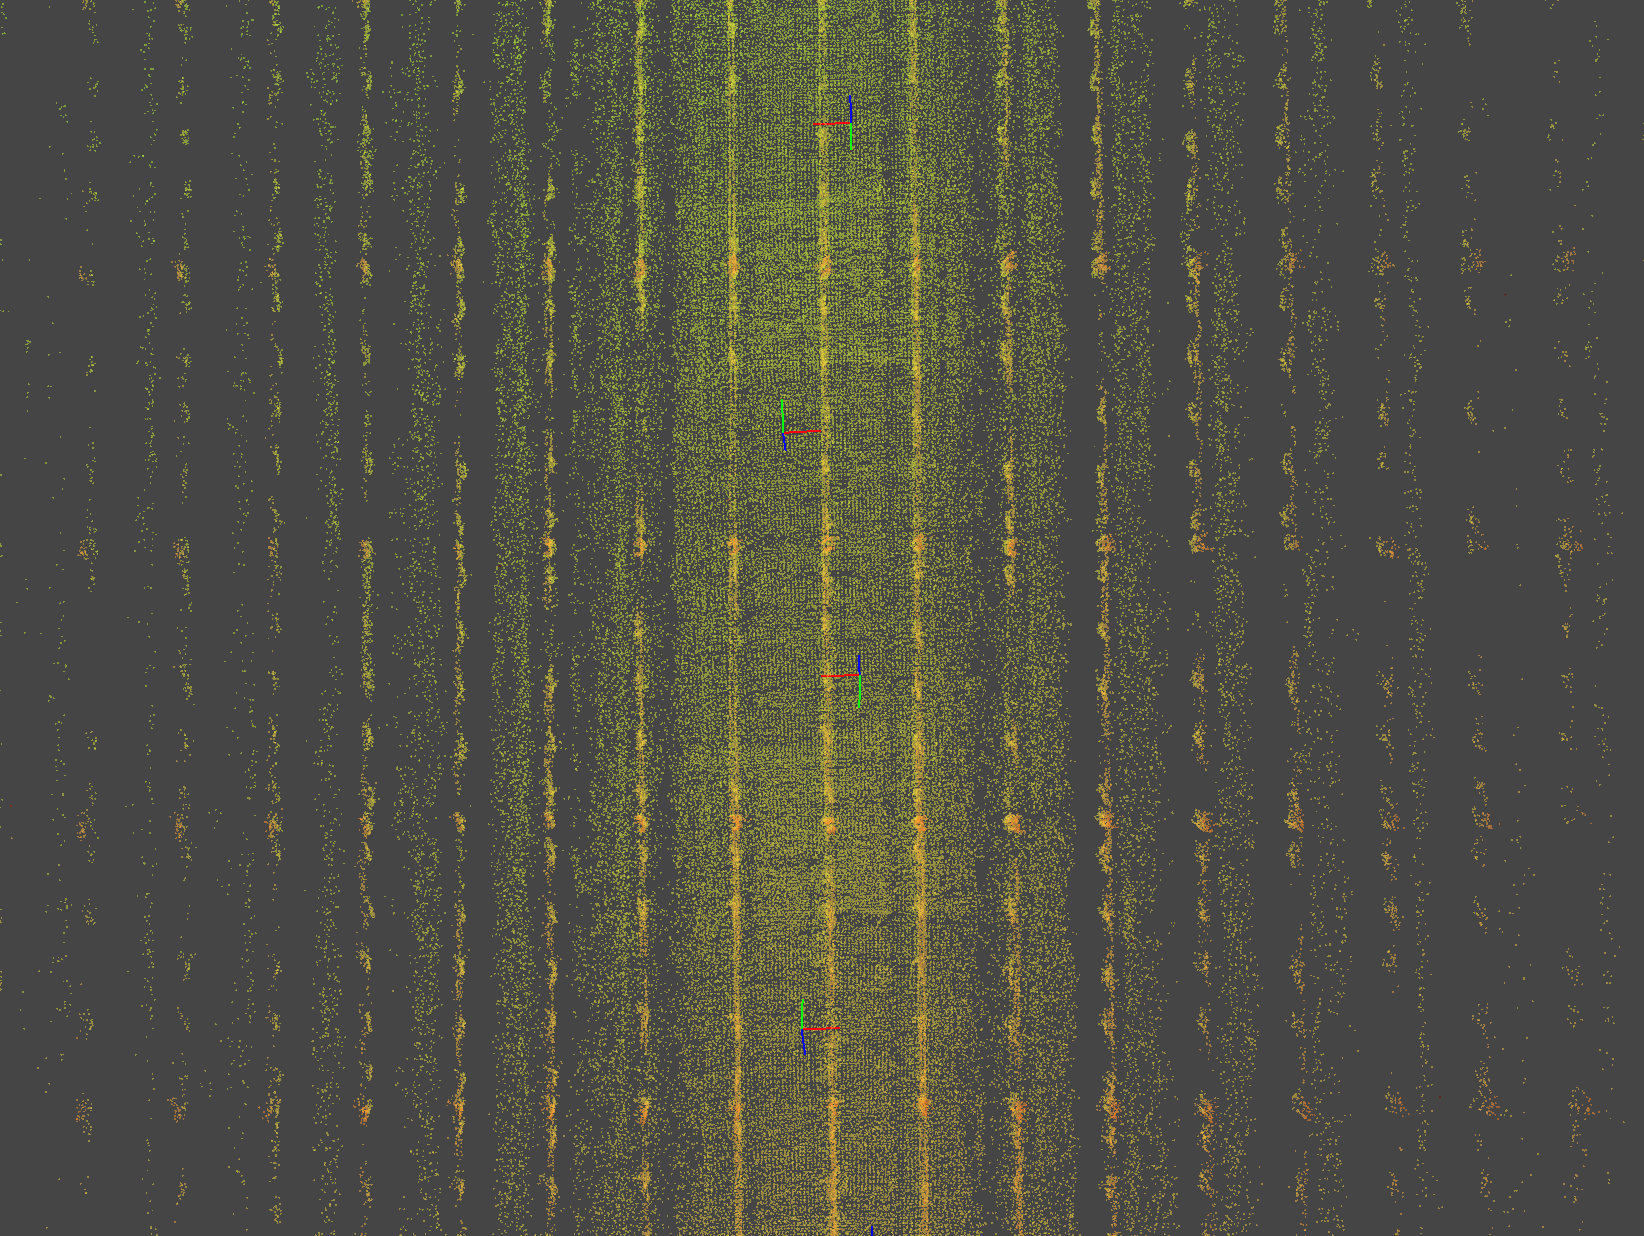
\includegraphics[width=0.85\linewidth]{3-SLAM/3-discussion/figures/zoomed_in_rows_SLAM_map.png}
    \caption{Bird's-eye view of the LiDAR point cloud map captured in the UCVision vineyard. The repetitive, corridor-like geometry of the rows is clearly visible: each row presents an identical wall of vegetation returns, with no distinctive geometric feature to discriminate one row from another. This perceptual aliasing is the root cause of the row-skipping failure described above.}
    \label{fig:zoomedRowsSLAMMap}
\end{figure}

\subsection{Refined GLIM Performance}
\label{subsec:slam-discussion-refined}

The transition from the baseline GLIM algorithm to the refined (parameterised) version demonstrates a marked improvement in localisation stability and drift suppression. While the baseline algorithm frequently succumbed to the failure modes described in previous sections, the refined version exhibits a more controlled error accumulation. Full performance metrics for all datasets are reported in \cref{tab:refined_performance}.

The most prominent improvement is observed in the \textit{error percent per metre} metric. In the baseline configuration, Dataset 2 exhibited a peak error of 7.3610\%, whereas the refined version reduced this to 3.6150\%, a reduction of approximately 50\%. In more favourable conditions, such as Dataset 4, the error dropped from 4.1910\% in the baseline to 0.6680\% in the refined version. This indicates that parameter optimisation effectively mitigates the ``point of no return'' by maintaining better geometric alignment over longer durations.

The \textit{RPE 1\,m translation standard deviation} serves as a proxy for the ``smoothness'' or ``jitter'' of the trajectory. While the baseline GLIM suffered from jagged trajectories around points of failure, peaking at a standard deviation of 0.9384 in Dataset 3, the refined GLIM consistently lowered this jitter across all datasets. For example, in Dataset 3, the refined version achieved an RPE standard deviation of 0.8239. The overall reduction suggests that the optimised parameters facilitate more reliable and consistent scan-matching, reducing the frequency of the ``jumps'' caused by false-positive matches in repetitive environments.

The \textit{error per metre (m)} metric further reinforces these findings. The refined GLIM consistently achieved sub-centimetre drift per metre in datasets where the baseline was drifting several centimetres (e.g., Dataset 0 dropping from 0.0340~m to 0.0087~m). This suggests that the refinement process successfully tuned the SLAM parameters to better suit the specific LiDAR characteristics and environment structure, delaying the onset of the catastrophic failures observed in the baseline.

\begin{table}[htbp]
\centering
\caption{Comparative Performance: Baseline vs. Refined GLIM}
\label{tab:comparison_summary}
\begin{tabularx}{\textwidth}{lXXXXX}
\toprule
\textbf{Metric} & \textbf{Dataset 0} & \textbf{Dataset 1} & \textbf{Dataset 2} & \textbf{Dataset 3} & \textbf{Dataset 4} \\ \midrule
\textbf{Error \% Reduction} & 73.9\% & 51.4\% & 50.8\% & 84.6\% & 84.0\% \\
\textbf{RPE Std Improvement} & 12.2\% & 5.8\% & 28.8\% & 12.2\% & 19.9\% \\ \bottomrule
\end{tabularx}
\end{table}

\subsection{GLIM-GNSS: GNSS-Augmented Localisation}

By introducing a source of absolute positional observability absent from both the baseline and refined GLIM configurations, GLIM-GNSS eliminates the unbounded drift inherent in scan-matching-only odometry. The resulting improvement is approximately two orders of magnitude in localisation accuracy relative to the untuned GLIM baseline (0.015–0.050\% vs.\ 1.3–7.4\%), and approximately one order of magnitude relative to the refined GLIM (0.015–0.050\% vs.\ 0.6–3.6\%). It is important to note that this comparison is not purely algorithmic: GLIM-GNSS leverages sparse GNSS factor injection as an additional sensor input, providing absolute positional observability that is unavailable to both the baseline and refined configurations. The improvement therefore reflects the combined effect of GNSS integration and parameter optimisation, rather than algorithmic changes alone. The GLIM-GNSS system's error percentage per metre ranges from $0.0153\%$ (Dataset 4) to $0.0501\%$ (Dataset 2) (see \cref{tab:proposed_performance}), compared to the refined GLIM's range of $0.6081\%$ to $3.6150\%$. This reduction is consistent across all datasets, with no observable catastrophic failure modes analogous to those seen in earlier iterations.

\subsubsection{GNSS Integration}

Whereas baseline GLIM operates exclusively on scan-matching odometry, GLIM-GNSS augments the submaps and keyframes' local relative information with periodic absolute position measurements from the GNSS receiver. This integration serves two distinct functions: (1) it grounds the map frame in a fixed real-world coordinate system, ensuring trajectory estimates are metrically consistent with the farm's local ENU reference rather than an arbitrary per-run origin; and (2) because GNSS measurements enter as factors in a graph optimiser rather than as Kalman filter updates, their effect propagates non-causally, correcting prior states within the optimisation window rather than only conditioning future estimates.

The effectiveness of this approach is evident in comparing error accumulation results. In the refined GLIM, even with parameter optimisation, the error percent per metre remains linear or superlinear across the traversal. By contrast, GLIM-GNSS maintains sub-centimetre per-metre errors throughout, suggesting that the global constraints are sufficiently frequent and accurate to prevent drift from establishing itself in the first place.

This result is further reinforced by the GNSS factor utilisation statistics (\cref{tab:gnss_stats}): across all datasets, between 0.65--0.78\% of all available GNSS data points were injected into the factor graph following outlier rejection. This sparsity is itself a key achievement of this work. A primary motivation for the GLIM-GNSS architecture was to reduce operational dependence on RTK-GNSS, which is subject to signal degradation from canopy occlusion, multipath interference, and adverse weather, as well as high infrastructure costs in agricultural deployments. The results demonstrate that the vast majority of localisation accuracy is recovered through the LiDAR-inertial odometry backbone, with GNSS contributing only infrequent global anchors to prevent long-term drift accumulation. Achieving one to two orders of magnitude improvement over the baseline and refined GLIM configurations, respectively, at sub-percent GNSS utilisation confirms that dense or continuous RTK coverage is not a prerequisite for precise trajectory estimation in the GLIM-GNSS architecture.

\subsubsection{Dataset-Specific Performance Variability}

Despite the strong performance of GLIM-GNSS across all datasets, performance does vary across datasets in a pattern that suggests environmental factors influencing localisation quality. Dataset 2 exhibits the highest error metrics (0.0501\% error per metre, RMSE $y$ of 0.2003~m, ATE of 0.1741~m), whereas Dataset 3 achieves the lowest error (0.0134\% error per metre) and Dataset 1 the second lowest (0.0154\%). 

The degradation in Dataset 2 is likely due to environmental conditions rather than algorithmic limitations. Dataset 2 also recorded the fewest raw GNSS measurements prior to outlier rejection (7,236 points, compared to 9,241--13,461 across the remaining datasets; see \cref{tab:gnss_stats}), providing independent evidence of reduced signal availability rather than merely an elevated rejection rate. The low factor utilisation (0.65\% of available GNSS data points injected into the factor graph, the lowest across all datasets) is therefore consistent with canopy occlusion or multipath interference reducing the absolute number of receivable signals along that route. The geometric consistency-based outlier rejection, whilst effective at filtering genuinely erroneous points, cannot recover lost signal availability. Even under these challenging conditions, the localisation error remained controlled at $0.0501\%$, indicating robustness to transient GNSS degradation.

\subsubsection{Relative Pose Error}

The Relative Pose Error (RPE) metrics, which assess the consistency of local pose increments, provide insight into frame-to-frame localisation smoothness. GLIM-GNSS achieves RPE 1~m translation standard deviations ranging from $0.0205$ to $0.0479$~m across all datasets, compared to the refined GLIM's $0.2449$ to $0.8239$~m. This roughly tenfold to thirty-fivefold reduction in local pose jitter indicates that the global constraints are not merely correcting large-scale drift, but are improving the consistency of short-horizon relative measurements.

This improvement likely arises from the factor graph's ability to reason about odometric uncertainty jointly with global constraints. When the optimiser encounters a region where local odometry is inconsistent with global GNSS observations, it propagates the correction smoothly across the pose graph rather than applying isolated jump corrections. This smoothness is essential for downstream applications such as robotic arm control, where abrupt discontinuities in perceived position could cause trajectory tracking errors.

\subsubsection{GASP Metric Behaviour and Optimisation Dynamics}

A counterintuitive finding is a marginal upward trend in the GASP (Global Alignment and Smoothness Profile) metric for the single best-performing run across the four parameter optimisation stages (\cref{fig:comparison_progression}). Unlike the baseline GLIM error percentage, which exhibits clear convergence and monotonic improvement (\cref{fig:baseline_progression,fig:baseline_error_dist}), the GLIM-GNSS system's best-run GASP metric increases (degrades) marginally from stage one to stage four (\cref{fig:proposed_progression}). This trend could be due to the stochastic nature of the Latin Hypercube parameter search rather than to any systematic degradation. The differences between near-optimal configurations are negligible, and stage one may have already identified a configuration that performs near-optimally. Subsequent stages sample nearby regions of the parameter space and, by chance, return configurations that score marginally worse on GASP. The magnitude of the variation is small enough that it falls within the expected noise of the pseudo-random search process.

Despite this marginal decline in peak performance, the overall distribution of GASP metric values improves significantly across the four stages, as shown in \cref{fig:comparison_dist}. As shown in \cref{fig:proposed_error_dist}, the error distributions shift progressively leftward over successive stages, indicating an improvement in typical performance. Concurrently, the distributions become taller and narrower — that is, the standard deviation decreases — reflecting an increase in the reliability and consistency of results. In contrast, the stage zero distribution is comparatively flat and wide, indicating that results at that stage were highly variable and unpredictable. This evolution demonstrates that the optimisation process is not identifying a single lucky configuration, but is systematically converging the parameter space towards a regime in which good performance is reproducible. The trade-off between peak and median performance is therefore a natural consequence of this convergence: as the search focuses on consistently high-performing regions, extreme but unreliable high-performing outliers are replaced by a tighter cluster of reliably good solutions.

\subsection{Comparative Analysis and Mechanisms of Improvement}

The experimental results, summarised in \cref{tab:comparison_table_key_metrics} and visualised across all metrics and datasets in \cref{fig:comparison_spider}, reveal a clear hierarchy of performance and illustrate the mechanisms driving improvements at each stage.

\subsubsection{Parametrisation vs. Sensor Fusion}

The transition from baseline to refined GLIM demonstrates that parameter tuning can reduce error magnitude significantly (50--85\% reduction in error percentage per metre; see \cref{fig:spider_ep} and \cref{fig:spider_epm}). However, parameter optimisation alone does not eliminate the fundamental instability of scan-matching-only odometry in repetitive vineyard environments. The refined GLIM still exhibits occasional trajectory inconsistencies and elevated RPE and ATE metrics relative to GLIM-GNSS (see \cref{fig:spider_RPE_std} and \cref{fig:spider_ATE}).

By contrast, the transition from refined GLIM to the GNSS-augmented GLIM-GNSS represents a qualitative shift in localisation architecture. Rather than optimising the tuning parameters of a single sensor modality, GLIM-GNSS introduces a fundamentally independent source of global position information. This architectural change achieves improvements that parametrisation alone cannot reach. The reduction in error percentage per metre from refined GLIM to GLIM-GNSS ($\sim$97--99\%) is larger and more consistent than the corresponding improvement from baseline to refined GLIM ($\sim$51--85\%), and GLIM-GNSS exhibits no dataset in which performance degrades significantly.

\subsubsection{Role of Outlier Rejection}

The geometric consistency-based outlier rejection procedure is critical in ensuring that only reliable GNSS measurements are incorporated into the factor graph. This aggressive filtering makes the sparse utilisation viable; by ensuring that every incorporated constraint is geometrically consistent, the procedure prevents a single erroneous global measurement from corrupting the factor graph. The architecture therefore achieves the desired property of sparse GNSS integration, using the global sensor as an infrequent but reliable anchor for the scan-matching-based odometry. This deterministic filtering approach, based on rigid-body distance preservation, is well-suited to the repetitive vineyard environment, where probabilistic alternatives such as RANSAC would require outlier distribution assumptions that may not hold in structured agricultural settings.

The robustness of this design is confirmed by Dataset 2, where GNSS factor utilisation falls to its lowest observed value of 0.65\%, yet localisation error remains controlled at $0.0501\%$ per metre. This indicates that each geometrically verified constraint carries sufficient positional information to anchor the trajectory even when GNSS availability is degraded.

\subsection{Generalisation to the Evaluation Dataset}
\label{subsec:slam-generalisation}

Beyond performance on the parameterisation datasets, the three configurations were evaluated on a held-out Evaluation Dataset to assess whether the observed improvements are specific to the training data distribution or generalise to previously unseen routes. The results are reported in \cref{subsec:slam-eval-results}; the analysis here focuses on what they reveal about generalisation behaviour.

\subsubsection{Overall Performance Hierarchy}

The three-tier performance ranking observed across the parameterisation datasets — baseline GLIM performing worst, refined GLIM intermediate, and GLIM-GNSS achieving the lowest errors — is broadly preserved on the Evaluation Dataset (see \cref{tab:eval_comparison_key_metrics}). The ordering holds for error percentage per metre and error per metre. For RPE 1\,m translation standard deviation, however, the refined GLIM's mean (0.4019) exceeds that of the baseline (0.1093) due to the influence of at least one catastrophic failure run, which inflates the aggregate statistic beyond the baseline's more uniformly distributed error. GLIM-GNSS achieves the lowest value on all three metrics. This overall consistency indicates that neither the parameterisation process nor the GNSS integration architecture produces results that are specific to the routes on which they were developed.

\subsubsection{Baseline GLIM}

The baseline GLIM mean error percentage per metre on the Evaluation Dataset falls within the range observed on the parameterisation datasets (1.253\%--7.361\%) and is comparable to the middle-tier parameterisation datasets (see \cref{tab:eval_baseline_performance}), indicating no systematic degradation on unseen data. This is expected: the baseline configuration involves no parameter tuning, so there is no mechanism by which its behaviour could be route-specific. The modest run-to-run variability is consistent with the stochastic nature of the scan-matching front-end.

\subsubsection{Refined GLIM}

The mean error percentage per metre for the refined GLIM on the Evaluation Dataset is consistent with the parameterisation dataset range (0.608\%--3.615\%), indicating that the optimised parameters transfer well in terms of mean performance (see \cref{tab:eval_refined_performance}).

Nonetheless, the results also reveal a significant instability that is not captured by the mean error percentage alone. As reported in \cref{tab:eval_refined_performance}, the maximum 3D positional error exhibits a mean--median discrepancy of approximately threefold (39.59\,m vs.\ 13.09\,m), with a maximum observed value of 148.61\,m. This pattern indicates that at least one of the five runs experienced a catastrophic failure of the type described in \cref{subsec:slam-discussion-refined} — a sudden and irrecoverable collapse of scan-matching alignment leading to unbounded planar drift. The same failure signature is visible in the RPE metrics, where mean values are an order of magnitude larger than the corresponding medians, confirming that the elevated aggregates are driven by a tail event rather than uniformly elevated error.

This apparent bimodal behaviour — the majority of runs performing well, with an occasional catastrophic failure — is arguably a more concerning failure mode in practice than a uniformly elevated error, because it is unpredictable at deployment time. The small sample size ($n = 5$) limits formal distributional characterisation, but the magnitude of the outlier (max positional error exceeding the median by a factor of eleven) is sufficient to establish that the failure mode persists on unseen routes. An operator relying on the refined GLIM cannot distinguish an impending failure run from a well-behaved one prior to the failure event. The parameter optimisation delays the onset of the instability described in the parameterisation dataset analysis but does not eliminate the underlying scan-matching vulnerability in semi-structured vineyard environments. Whether the catastrophic run can be attributed to specific environmental factors along the Evaluation Dataset route — such as a stretch of low-geometric-excitation terrain or a section with reduced inter-row distinctiveness — cannot be determined from aggregate statistics alone and would require per-run trajectory inspection.

\subsubsection{GLIM-GNSS}

The GLIM-GNSS system's Evaluation Dataset performance falls within and is consistent with the parameterisation dataset range of 0.0153\%--0.0501\% for error percentage per metre (see \cref{tab:eval_proposed_performance}). The standard deviation across five runs is less than 2.5\% of the mean value, indicating near-deterministic behaviour. This contrasts sharply with the refined GLIM, where the corresponding metric standard deviation accounts for approximately 17.5\% of the mean. The GASP metric likewise falls within the parameterisation dataset range (0.0274--0.0679), confirming consistent behaviour on both local and global accuracy dimensions.

This near-deterministic behaviour confirms a practically important property of the GLIM-GNSS architecture: the GNSS global constraint effectively suppresses the non-deterministic component of the underlying odometry pipeline. An operator deploying the system can therefore expect consistent performance across repeated runs rather than a distribution of outcomes that may occasionally include a failure event.

The error percentage per metre on the Evaluation Dataset is directly comparable to the parameterisation results, with no evidence of performance degradation on held-out data. Since the Evaluation Dataset was collected at the same farm, these results demonstrate route-level rather than cross-environment generalisation.

\subsection{Limitations and Implications for Vineyard Robotics}

The GLIM-GNSS system's consistent sub-centimetre drift rate (error per metre of traversal) has direct implications for robotic pruning feasibility. This per-metre drift must be distinguished from absolute trajectory error: while the per-metre error remains below 1~mm across all datasets, the cumulative position error over a full traversal reaches approximately 0.7--1.0~m. Pruning tasks require localisation accuracy sufficient to position the robotic arm within reach of target vine structures. With typical vine stems ranging from 5--15~mm in diameter, this absolute error bound can be accommodated through local perception-based arm guidance or online trajectory adjustment based on close-range stereo or depth sensing.

A fundamental limitation of the evaluation presented in this chapter is that all reported metrics are restricted to translational quantities: ATE measures absolute positional accuracy relative to ground truth, RPE and error per metre quantify relative translational drift, and the Global Alignment and Smoothness Profile (GASP) combines normalised drift rate and translational RPE standard deviation into a single relative performance index. The evaluation does not assess rotational pose accuracy (roll, pitch, and yaw). For high-level navigation and path planning, translational accuracy is the primary concern, and the reported results are sufficient to characterise coarse localisation quality. However, for fine-grained manipulation tasks such as autonomous pruning, the full six-degree-of-freedom pose of the robot relative to a vine structure is required. A position estimate that is globally accurate but accompanied by an unquantified orientation error may still be insufficient to guide a robotic arm to within the centimetre-level precision needed to interact with individual vine shoots.

A second methodological consideration is that the ground truth trajectory used for evaluation is itself derived from real-time RTK-GNSS fixes, while GLIM-GNSS also incorporates GNSS measurements as sparse factors. This apparent circularity does not invalidate the evaluation for two reasons: (1)~the ground truth uses the complete, continuous RTK fix stream at full receiver rate, whereas GLIM-GNSS injects fewer than 1\% of available GNSS fixes as discrete factor-graph constraints after geometric outlier rejection; the information content available to each is therefore fundamentally different; and (2)~the primary comparison is between GLIM-GNSS and the refined GLIM, which shares the same ground truth but receives no GNSS input, isolating the effect of sparse GNSS integration on localisation accuracy.

In summary, the experiments in this chapter establish a three-tier performance hierarchy: the baseline GLIM algorithm exhibits unbounded drift in repetitive vineyard environments, the refined GLIM partially suppresses this instability through parameter optimisation but remains susceptible to catastrophic failure, and GLIM-GNSS achieves consistent sub-centimetre per-metre drift rates by grounding the factor graph with sparse but geometrically verified global constraints. This hierarchy is preserved on a held-out evaluation route, where GLIM-GNSS exhibits near-deterministic behaviour in contrast to the stochastic failure distribution of the refined GLIM. The principal gap in this evaluation, specifically unquantified rotational accuracy, directly motivates the fine-grained alignment approach presented in the following chapter.

Chapter~4 addresses this limitation by evaluating precise alignment techniques that estimate the full six-degree-of-freedom robot pose relative to a pre-existing 3D model of the vine structure, operating with no additional GNSS input and using local dense perception to constrain pose estimation.